\documentclass[12pt]{article}
\usepackage{graphicx}
\usepackage{wrapfig}
\usepackage{tikz}
\usepackage{ucs} 
\usepackage[T1,T2A]{fontenc}
\usepackage[utf8x]{inputenc} % Включаем поддержку UTF8  
\usepackage[russian]{babel}  % Включаем пакет для поддержки русского языка  
\usepackage{amsfonts}
\usepackage[left=1.5cm,right=1.5cm]{geometry}
\usepackage{amsmath}
\usepackage{amssymb}
\DeclareMathOperator\arctanh{arctanh}

\usetikzlibrary{decorations.markings}
\usetikzlibrary{patterns}
\usetikzlibrary{calc}
\usetikzlibrary{arrows}
\title{Задачи к 9 лекции}  
\author{Нечитаев Дмитрий}

\begin{document} 
	\maketitle
	\section*{Задача 1}
	Необходимо получить уравнения на медленные переменные в задаче Кеплера, предполагая, что частица находится в среде со слабым трением.
	\[\mathbf{F_{ad}} = -\nu \mathbf{\dot{r}} \eqno(1)\]
	
	
	Запишем уравнение движения частицы:
	\[m\mathbf{\ddot{r}} = -\frac{\alpha}{r^3}\mathbf{r} - \nu \mathbf{\dot{r}} \eqno(2)\]
	На временах порядка нескольких периодов $\textbf{r}$ ведет себя как и в невозмущенной задаче Кеплера, значит данную функцию можно разложиьт в ряд фурье:
	\[\mathbf{r} = \mathbf{r_0} + \sum_{n=1}^{\infty} \mathbf{a_n} \cos(n\omega t )+\mathbf{b_n}\sin(n\omega t) \eqno(3)\]
	После дифференцирования по времени постоянный вектор $\mathbf{r_0}$ исчезает, а это значит, что скорость частицы $\mathbf{v} = \mathbf{\dot{r}}$ при усреднении по периоду будет давать 0.
	Из этого можно заключить, что если усреднить уравнение движения (2) по периоду, то последнее слагаемое обнулится, т.е. имеет место соотношение:
	\[\Big<m\mathbf{\ddot{r}}\Big>_T = -\Big<\frac{\alpha}{r^3}\mathbf{r}\Big>_T \eqno(4)\]
	
	
	Перейдем к исследованию эволюции медленных переменных. На лекции было получено соотношение для производных момента импульса и вектора Лапласа-Рунге-Ленца:
	\[\mathbf{\dot{M}} = \mathbf{r}\times\mathbf{F_{ad}},\;\;\;\;\;\mathbf{\dot{A}} = \frac{1}{\alpha m} \mathbf{F_{ad}}\times \mathbf{M} + \frac{1}{\alpha} \mathbf{\dot{r}}\times\Big(\mathbf{r}\times\mathbf{F_{ad}}\Big) \eqno(5)\]
	
	Переходим к средним значениям:
	\[\mathbf{\dot{M}} = -\nu\Big<\mathbf{r}\times\mathbf{\dot{r}} \Big>_t = -\frac{\nu}{m} \Big< \mathbf{r}\times\mathbf{m\dot{r}}\Big>_T = -\frac{\nu}{m}\Big<\mathbf{M}\Big>_T \eqno(6)\]
	В силу того, что переменная $\mathbf{M}$ является медленной, то считаем, что за период $T$ момент импульса практически не меняется. Таким образом получаем соотношение:
	\[\mathbf{M}(t) = -\frac{\nu}{m}\mathbf{M} \eqno(7)\]
	Интегрирование дает нам соотношение для момента импульса:
	\[\mathbf{M}(t) = \mathbf{M_0}\exp\Big(-\frac{\nu}{m} t\Big) \eqno(8)\]
	Разберемся теперь как эволюционирует вектор Рунге-Ленца:
	\[\mathbf{\dot{A}} = -\Big< \frac{1}{\alpha m} \mathbf{\nu \dot{r}} \times \mathbf{M}\Big>_T + \frac{1}{\alpha}\Big<\mathbf{\dot{r}} \times \Big( \mathbf{r} \times \mathbf{(-\nu \dot{r})}\Big)\Big>_T = \]
	\[= - \Big< \frac{1}{\alpha m} \mathbf{\nu \dot{r}}\Big>_T \times \mathbf{M} + \frac{1}{\alpha}\Big<\mathbf{\dot{r}}  \times \mathbf{M} \Big>_T = \frac{1}{\alpha}\Big<\mathbf{\dot{r}}\Big>_T  \times \mathbf{M} = 0 \eqno(9)\]
	Получается что вектор $\mathbf{A}$ остается постоянным. Если обратиться к геометрическим параметрам орбиты, то получим, что эксцентреситет, равный $|\mathbf{A}|$ остается постоянным, а параметры орбиты, пропорциональный $\mathbf{M}^2$ задающий "размеры" траектории убывает со временем как $\sim \exp\Big(-2\frac{\nu}{m} t\Big)$. Т.е тело движется по подобным эллипсам, размеры которых убывают экспоненциально со временем.
	
	\pagebreak
	В классической задаче Кеплера траектория в полярной системе координат определяется выражением:
	\[r(\phi) = \frac{p}{1+A\cos\phi},\;\;\; p = \frac{M^2}{\alpha m} \eqno(10)\]
	Посчитаем период обращения тела по такой траектории:
	\[T = \int_0^T dt = \int_0^{2\pi} \frac{d\phi}{\phi_t'} = \int_0^{2\pi} \frac{mr^2}{M^2}d\phi = \frac{mp^2}{M}\int_0^{2\pi} \frac{d\phi}{(1+A\cos \phi)^2} \eqno(11)\]
	\[J(\beta) = \int_0^{2\pi} \frac{dx}{\beta+A\cos x} = \left\{ t = \tan(x/2)\right\} =  2 \int_0^{\infty} \frac{2dt}{\beta(1+t^2)+A(1-t^2)} = 4 \int_0^{\infty} \frac{dt}{(A+\beta) + t^2 (\beta-A)} =  \]
	\[ = \frac{4}{\beta-A} \int_0^{\infty} \frac{dt}{\frac{A+\beta}{\beta-A} + t^2} = \frac{2\pi}{\sqrt{\beta^2-A^2}} \eqno(12)\]
	Для вычисления интеграла, который фигурирует в (15) необходимо взять производную $\partial_\beta J(\beta) \Big|_{\beta = 1}$
	\[\partial_\beta J(\beta) \Big|_{\beta = 1} = -\frac{2\pi\beta}{(\beta^2-A^2)^{3/2}} \Big|_{\beta = 1} = -\frac{2\pi}{(1-A^2)^{3/2}} \eqno(13)\]
	Это выражение соответствет интегралу:
	\[ \partial_\beta J(\beta) = -\int_0^{2\pi} \frac{dx}{(\beta+A\cos x)^2} \eqno(14)\]
	С учетом выражения (16), (17) находим выражение для периода из формулы (15):
	\[\boxed{T = \frac{mp^2}{M}\cdot \frac{2\pi}{(1-A^2)^{3/2}}} \eqno(15)\]
	\section*{Задача 2}
	В данной задаче требуется определить как будет изменяться траектория частицы, если учесть, что происходит потеря массы из-за излучения.
	
	
	Первым делом определим внешнюю силу, которая действует на частицу, для этого запишем теорему об изменении количества движения:
	\[\frac{d\mathbf{Q}}{dt} = -\frac{\alpha \mathbf{r}}{r^3} \Leftrightarrow \dot{m}\mathbf{\dot{r}} + m\mathbf{\ddot{r}} = -\frac{\alpha \mathbf{r}}{r^3} \Leftrightarrow \]
	\[m\mathbf{\ddot{r}} = -\frac{\alpha \mathbf{r}}{r^3} - \dot{m}\mathbf{\dot{r}} \eqno(1)\]
	\pagebreak
	
	Исследуем как меняется момент импульса. С учетом формулы (1) получаем:
	\[\mathbf{M} = m\mathbf{r}\times\mathbf{\dot{r}} \Rightarrow \mathbf{\dot{M}} = m \mathbf{r}\times\mathbf{\ddot{r}} = -\dot{m} \mathbf{r}\times\mathbf{\dot{r}} = -\frac{\dot{m}}{m} \mathbf{M} \eqno(2)\]
	Важно заметить, что $\mathbf{M}$ --- это момент импульса только планеты, поэтому при посчете производной член, содержащий $\dot{m}$ мы не учитывали, т.к. в таком случае получили бы изменение импульса системы: планета + излученное вещество. Из формулы (1) видно, что на такую систему действует только одна центральная сила, а значит и изменение момента импульса относительно центра поля будет нулевым.
	
	Теперь обратимся к вектору Рунге-Ленца:
	\[\mathbf{A} = \frac{1}{\alpha} \mathbf{\dot{r}}\times \mathbf{M} - \frac{\mathbf{r}}{r} \eqno(3)\]
	Дифференцируем по времени:
	\[\mathbf{\dot{A}} = -\frac{\dot{\alpha}}{\alpha^2} \mathbf{\dot{r}}\times\mathbf{M} + \frac{1}{\alpha} \mathbf{\ddot{r}}\times \mathbf{M} + \frac{1}{\alpha} \mathbf{\dot{r}}\times\mathbf{\dot{M}} - \frac{\mathbf{\dot{r}}}{r} + \frac{\mathbf{r}\dot{r}}{r^2} = \]
	\[ = -\frac{\dot{\alpha}}{\alpha^2} \mathbf{\dot{r}}\times\mathbf{M} - \Big\{ \frac{1}{\alpha} \frac{\alpha \mathbf{r}}{r^3} \times (\mathbf{r}\times\mathbf{\dot{r}}) + \frac{\dot{m}}{\alpha} \mathbf{\dot{r}} \times (\mathbf{r}\times\mathbf{\dot{r}}) \Big\} - \frac{\dot{m}}{\alpha m}\mathbf{\dot{r}}\times\mathbf{M}- \frac{\mathbf{\dot{r}}}{r} + \frac{\mathbf{r}\dot{r}}{r^2} = \]
	\[= -\frac{\dot{\alpha}}{\alpha^2} \mathbf{\dot{r}}\times\mathbf{M} - \frac{2\dot{m}}{\alpha m}\mathbf{\dot{r}}\times\mathbf{M} = -\Big(\frac{\dot{\alpha}}{\alpha^2}+\frac{2\dot{m}}{\alpha m}\Big)\mathbf{\dot{r}}\times\mathbf{M} \eqno(4) \]
	
	Произведем усреднение выражений (2) и (4), учитывая, что\footnote{Данные соотношения показывают, что за время периода величины $\alpha,m$ практически не изменаются} $T\dot{\alpha}/\alpha,T\dot{m}/m \ll 1$, где $T$ --- период обращения.
	\[\mathbf{\dot{M}} = -\Big<\frac{\dot{m}}{m}\Big>_T\mathbf{M} = - \frac{\dot{m}}{m} \mathbf{M} \eqno(5)\]
	\[\mathbf{\dot{A}} = -\Big<\Big(\frac{\dot{\alpha}}{\alpha^2}+\frac{2\dot{m}}{\alpha m}\Big)\mathbf{\dot{r}}\Big>_T \times \mathbf{M} = -\Big(\frac{\dot{\alpha}}{\alpha^2}+\frac{2\dot{m}}{\alpha m}\Big) \Big<\mathbf{\dot{r}}\Big>_T\times\mathbf{M} = \mathbf{0}\eqno(6)\]
	
	
	Получается, что т.к. планета теряет массу, то $\dot{m}/m <0$ т.е. момент импульса экспоненциально растет, а значит характерный размер орбит возрастает как $\sim \exp(-2\frac{\dot{m}}{m}t)$. Причем эксцентриситет орбиты остается постоянным.
	
	\pagebreak
	\section*{Задача 3}
	Исследуем траекторию электрона в поле протона при добавлении слабого магнитного поля.
	
	
	Уравнение движения электрона:
	\[m\mathbf{\ddot{r}} = - \frac{\alpha \mathbf{r}}{r^3} -e\mathbf{\dot{r}}\times\mathbf{B} \eqno(1)\]
	Производные векторов $\mathbf{M},\mathbf{A}$:
	\[\mathbf{\dot{M}} = -e\mathbf{r}\times(\mathbf{\dot{r}}\times\mathbf{B})\;\;\;\;\mathbf{\dot{A}} = -\frac{e}{\alpha m} (\mathbf{\dot{r}}\times\mathbf{B}) \times \mathbf{M} - \frac{e}{\alpha} \mathbf{\dot{r}} \times \Big(\mathbf{r}\times (\mathbf{\dot{r}}\times\mathbf{B}) \Big)\eqno(2)\]
	
	Отметим пару тождеств:
	\[\mathbf{r}\times(\mathbf{\dot{r}}\times B) + \mathbf{\dot{r}}\times(\mathbf{r}\times \mathbf{B}) = \frac{d}{dt}\Big( \mathbf{r}\times(\mathbf{r}\times\mathbf{B}) \Big) \eqno(3)\]
	\[\mathbf{r}\times(\mathbf{\dot{r}}\times\mathbf{B}) + \mathbf{\dot{r}}\times(\mathbf{B}\times\mathbf{r}) + \mathbf{B}\times(\mathbf{r}\times\mathbf{\dot{r}}) = \mathbf{0} \eqno(4)\]
	В силу того, что поле слабое, можно считать $\mathbf{r}$ --- периодическая функция, а значит $\mathbf{r}\times(\mathbf{r}\times\mathbf{B})$ --- тоже периодическая функция, тогда среднее значение производной (3) за период будет равно нулю\footnote{Это утверждение доказывалось в первой задаче}. Тогда можно установить:
	\[\Big<\mathbf{r}\times(\mathbf{\dot{r}}\times B)\Big>_T = \Big<\mathbf{\dot{r}}\times(\mathbf{B}\times \mathbf{r})\Big>_T \eqno(5)\]
	Усредняя выражение (4), учитывая соотношение (5), получаем:
	\[2\Big<\mathbf{r}\times(\mathbf{\dot{r}}\times B)\Big>_T = -\Big<\mathbf{B}\times(\mathbf{r}\times\mathbf{\dot{r}})\Big>_T \eqno(6)\]
	Тепрь можно посчитать усреднение момента импульса за период:
	\[\mathbf{\dot{M}} = \frac{e}{2m}\Big<\mathbf{B}\times(m\mathbf{r}\times\mathbf{\dot{r}})\Big>_T = \frac{e}{2m}\mathbf{B}\times \mathbf{M} = \mathbf{\Omega}\times\mathbf{M} \eqno(7)\]
	Тут введено обозначение $\mathbf{\Omega} = \frac{e}{2m}\mathbf{B}$.
	
	
	Из выражения (7) понятно, что вектор $\mathbf{M}$ вращается с постоянной угловой скоростью $\mathbf{\Omega}$.
	\pagebreak
	
	Перепишем уравнение (2) еще раз:
	\[\mathbf{\dot{M}} = -e\mathbf{r}\times(\mathbf{\dot{r}}\times\mathbf{B})\;\;\;\;\mathbf{\dot{A}} = -\frac{e}{\alpha m} (\mathbf{\dot{r}}\times\mathbf{B}) \times \mathbf{M} - \frac{e}{\alpha} \mathbf{\dot{r}} \times \Big(\mathbf{r}\times (\mathbf{\dot{r}}\times\mathbf{B}) \Big)\eqno(2)\]
	С учетом выражения для $\mathbf{\dot{M}}$ из уравнения (2) получаем соотношение для производной вектора $\mathbf{A}$:
	\[\mathbf{\dot{A}} = -\frac{e}{\alpha m} (\mathbf{\dot{r}}\times\mathbf{B})\times \mathbf{M} + \frac{1}{\alpha} \mathbf{\dot{r}}\times\mathbf{\dot{M}} = -\frac{e}{\alpha m} (\mathbf{\dot{r}}\times\mathbf{B})\times \mathbf{M} + \frac{1}{\alpha} \mathbf{\dot{r}}\times\mathbf{\dot{M}} + \frac{1}{\alpha} \mathbf{\ddot{r}}\times\mathbf{M} - \frac{1}{\alpha} \mathbf{\ddot{r}}\times\mathbf{M} = \]
	\[= -\frac{e}{\alpha m} (\mathbf{\dot{r}}\times\mathbf{B})\times \mathbf{M} + \frac{d}{dt}\Big( \frac{1}{\alpha}\mathbf{\dot{r}}\times\mathbf{M}\Big) -\frac{1}{\alpha} \mathbf{\ddot{r}}\times\mathbf{M} \eqno(8)\]
	Первые два члена в сумме зануляются при усреднении по периоду обращения. Подробнее рассмотрим что происходит с последним челеном: если подставить вторую производную из уравнения движения и усреднить полученный результат, то понятно, что т.к. вектор $\mathbf{M}$ практически не изменяется, то среднее значение величины $\sim \mathbf{\dot{r}}\times\mathbf{M}$ будет нулевым, тогда верно соотношение:
	\[\Big<\mathbf{\ddot{r}}\times\mathbf{M}\Big>_T = \Big<\frac{\mathbf{r}}{\alpha r^3} \times \mathbf{M}\Big>_T \eqno(9)\]
	Теперь воспользуемся симметрией невозмущенной орбиты: для этого разложим вектор $\mathbf{r}$ на 2 компоненты, первая будет параллельна $\mathbf{A}$, вторая перпендикулярна. Т.к. орбиты планет в невозмущенной задаче являются эллипсами, а вектор $\mathbf{A}$ проведен из фокуса к перигею орбиты, то получается, что среднее значение величины $\sim \mathbf{r_{\perp}} \times \mathbf{M}$ будет равно 0. 
	\begin{figure}[h!]
		\center{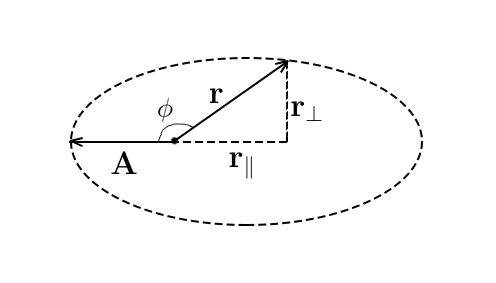
\includegraphics[scale=0.6]{orbit.png}}
		\caption{Примерная орбита планеты}
	\end{figure}

 	Получается что выражние (9) можно переписать в виде:
 	\[\Big<\mathbf{\ddot{r}}\times\mathbf{M}\Big>_T = \Big<\frac{\mathbf{r_\parallel}}{\alpha r^3} \times \mathbf{M}\Big>_T = \Big<\frac{r \cos\phi \mathbf{A}}{\alpha r^3 A}\Big>_T \times \mathbf{M} = \frac{1}{A\alpha} \Big<\frac{\cos \phi}{r^2}\Big>_T \mathbf{A\times M} \eqno(10)\]
 	Теперь считаем интеграл:
 	\[\Big<\frac{\cos \phi}{r^2}\Big>_T = \frac{1}{T}\int_0^{T} \frac{\cos \phi}{r^2} dt = \frac{1}{T} \int_0^{2\pi} \frac{\cos \phi}{r^2} \frac{d\phi}{\phi'_t} = \frac{1}{T} \int_0^{2\pi} \frac{\cos \phi}{r^2} \frac{r^2 m}{M}d \phi = 0 \eqno(11)\]
 	Возвращаясь по цепочке уравнений обратно к (2) делаем вывод, что вектор $\mathbf{A}$ является постоянной величиной.
 	
 	\section*{Задача 4}
 	На электрон действует сила $\mathbf{F}_{ad} = \beta \mathbf{\ddot{v}}$, где коэффициент $\beta = \frac{2e^2}{3c^3}$. Требуется определить что будет происходить с орбитой электрона и через какое время он упадет на протон.	
 	
 	Производная момента импульса записывается:
 	\begin{equation}
 	\mathbf{\dot{M}} = \mathbf{r\times F}_{ad}
 	\end{equation}
 	Пусть изначально электрон двигался по окружности, тогда его скорость определяется соотношением:
 	\begin{equation}
 	\mathbf{v} = \mathbf{\Omega \times r}
  	\end{equation}
  	Пренебрегая изменением $r$ за период находим соотношения для производных скорости:
  	\begin{equation}
  		\mathbf{\dot{v} = \Omega \times (\Omega \times r)}\;\;\;\;\mathbf{\ddot{v} = \Omega \times \dot{v}}
  	\end{equation}
  	Воспользуемся теперь тем фактом, что движение электрона будет плоским. Это утверждение очевидно, если сила является центральной, поэтому необходимо разобраться как добавочная сила $\mathbf{F}_{ad}$ влияет на момент импульса. Если отталкиваться от задачи Кеплера, то получим, что вектор $\mathbf{\ddot{v}}$ лежит в плоскости орбиты, причем он $\parallel \mathbf{v}$. Получается, добавочная сила меняет модуль момента импульса, и движение остается плоским. В таком случае можно переписать уравнение (3) через скалярные\footnote{Тут под $\omega$ подразумевается $|\mathbf{\Omega}|$} величины.
  	\begin{equation}
  		F_{ad} = \beta \omega^3 r
  	\end{equation}
  	В скалярном виде уранение (1) примет вид:
  	\[\frac{d}{dt}\Big( m r v \Big) = -\beta \omega^3 r \cdot r \Leftrightarrow\]
  	\begin{equation}
  		 \frac{d}{dt}\Big(m\omega r^2\Big) = -\beta \omega^3 r^2
  	\end{equation}
  	
  	Для определения зависимости радиуса от времени воспользуемся проекцией закона движения электрона на радиуальную ось:
  	\begin{equation}
  		m\omega^2 r = \frac{e^2}{r^2}
  	\end{equation}
  	Вытаскивем из этого соотношения $\omega$:
  	\begin{equation}
  		\omega = \frac{e}{r^{3/2}\sqrt{m} }
  	\end{equation}
  	Тогда подстановка в (5) дает соотношение:
  	\begin{equation}
  		\frac{d}{dt}\Big(e\sqrt{mr}\Big) = -\frac{\beta e^3r^2}{r^{9/2}m^{3/2}}
  	\end{equation}
  	Интегрируем уравнение (8):
  	\begin{equation}
  		\int_{R_0}^{0} \sqrt{r^5} d\sqrt{r} = -\int_0^{T} \frac{\beta e^2}{m^2} dt
  	\end{equation}
  	\begin{equation}
  		\frac{R_0^3}{6} = \frac{\beta e^2}{m^2}T \Leftrightarrow T = \frac{R_0^3m^2}{6e^2\beta} = \frac{R_0^3 m^2 3c^3}{12 e^4} = \frac{R_0^3 m^2c^3}{4e^4}
  	\end{equation}
  	Окончательно получаем:
  	\[\boxed{T = \frac{m^2c^3R_0^2}{4e^4}}\]
  	
  	
  	Теперь разберемся что происходит в процессе движения с вектором $\mathbf{A}$.
  	\begin{equation}
  		\mathbf{\dot{A} = }\frac{1}{\alpha m} \mathbf{F_{ad} \times M} + \frac{1}{\alpha} \mathbf{\dot{r}\times(r\times F_{ad}) }
  	\end{equation}
  	Первое слагаемое при усреденении дает 0, т.к. в $\mathbf{F}_{ad}$ сидит $\mathbf{\ddot{v}}$, которое является полной производной периодической функции. Для определения среднего значения второго члена выполним следующий ход:
  	\[\mathbf{\dot{r}\times (r\times F_{ad}) = \dot{r}\times \dot{M} = \dot{r}\times \dot{M} + \ddot{r} \times M - \ddot{r} \times M = \frac{d}{dt}\Big( \dot{r} \times M \Big)  - \ddot{r}\times M }\]
  	Получается, что усреднение по периоду дает соотношение:
  	\begin{equation}
  		\Big<\mathbf{\dot{r}\times (r\times F_{ad})}\Big>_T = -\Big<\mathbf{\ddot{r}\times M}\Big>_T = -\Big<\mathbf{\ddot{r}}\Big>_T\times \mathbf{M} = 0
  	\end{equation}
  	Последний переход в цепочке равенств (12) справедлив, т.к. электрон в невозмущенной задаче движется по окружности, а значит среднее ускорение будет нулевым.
  	
  	
  	Получается что вектор $\mathbf{A}$ остается постоянным в процессе движения электрона.
\end{document}